\documentclass[12pt,a4paper,oneside]{article}

\usepackage[utf8]{inputenc}
\usepackage[portuguese]{babel}
\usepackage[T1]{fontenc}
\usepackage{amsmath}
\usepackage{amsfonts}
\usepackage{amssymb}
\usepackage{graphicx}
\usepackage{xcolor}
% Definindo novas cores
\definecolor{verde}{rgb}{0.25,0.5,0.35}

\author{\\Universidade Federal de Goiás (UFG) - Regional  Jataí\\Bacharelado em Ciência da Computação \\Teoria da Computação \\Esdras Lins Bispo Jr.}

\date{28 de agosto de 2017}

\title{\sc \huge Prova (Parte 1)}

\begin{document}

\maketitle

{\bf ORIENTAÇÕES PARA A RESOLUÇÃO}

\small
 
\begin{itemize}
	\item A avaliação é individual, sem consulta;
	\item A pontuação máxima desta avaliação é 10,0 (dez) pontos, sendo uma das 06 (seis) componentes que formarão a média final da disciplina: quatro testes, uma prova e exercícios;
	\item A média final ($MF$) será calculada assim como se segue
	\begin{eqnarray}
		MF & = & MIN(10, S) \nonumber \\
		S & = & (\sum_{i=1}^{4} 0,2.T_i ) + 0,2.P  + 0,1.EA + EB\nonumber
	\end{eqnarray}
	em que 
	\begin{itemize}
		\item $S$ é o somatório da pontuação de todas as avaliações,
		\item $T_i$ é a pontuação obtida no teste $i$,
		\item $P$ é a pontuação obtida na prova,
		\item $EA$ é a pontuação total dos exercícios de aquecimentos, e
		\item $EB$ é a pontuação total dos exercícios-bônus.
	\end{itemize}
	\item O conteúdo exigido desta avaliação compreende o seguinte ponto apresentado no Plano de Ensino da disciplina: (1) Teoria da Computação, (2) Modelos de Computação e (3) Problemas Decidíveis.
\end{itemize}

\begin{center}
	\fbox{\large Nome: \hspace{10cm}}
\end{center}

\newpage

\begin{enumerate}
	
	\section*{Primeiro Teste}
	
	\item (5,0 pt) Esta questão diz respeito à MT $M_1$ cujo diagrama de estados, em sua versão simplificada, é apresentado na figura abaixo.	
	\begin{center}
		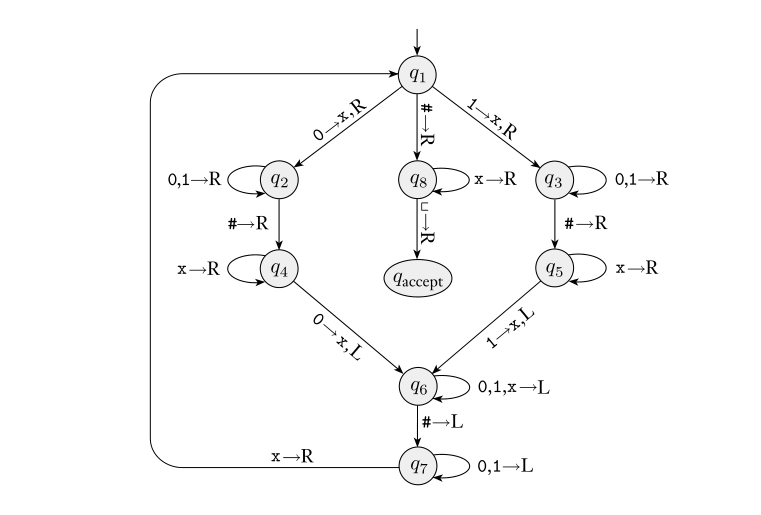
\includegraphics[width=\textwidth]{images/diagrama.png}
	\end{center}	
	 Dê a sequência de configurações nas quais $M_1$ entra quando iniciada sobre cada cadeia de entrada indicada nos itens abaixo:
	\begin{enumerate}
		\item $1\#1$
		\item $10\#11$
	\end{enumerate}
	
	\item (5,0 pt) Mostre que a classe de linguagens decidíveis é fechada sob a operação de concatenação. 
	
	\newpage
	
	\section*{Segundo Teste}
	
	\item (5,0 pt) Dê a descrição, em nível de implementação, da MT que decide a linguagem $A = \{\omega$ | $\omega$ contém duas vezes mais 0s que 1s$\}$. Admita que o alfabeto é o conjunto $\{0,1\}$.
	
	\item (5,0 pt) Considere o problema de se determinar se um AFD e uma expressão regular são equivalentes. Expresse esse problema como uma linguagem e mostre que ele é decidível.

\end{enumerate}

\section*{Teoremas Auxiliares}

\begin{itemize}
	
	\item[] {\bf Definição 1.16:} Uma linguagem é chamada de uma linguagem regular se algum autômato finito a reconhece.
	\item[] {\bf Teorema 1.25:} A classe de linguagens regulares é fechada sob a operação de união.
	\item[] {\bf Teorema 1.26:} A classe de linguagens regulares é fechada sob a operação de concatenação.
	\item[] {\bf Teorema 1.39:} Todo autômato finito não-determinístico tem um autômato finito determinístico
	equivalente.
	\item[] {\bf Teorema 1.49:} A classe de linguagens regulares é fechada sob a operação estrela.
	\item[] {\bf Teorema 1.54:} Uma linguagem é regular se e somente se alguma expressão regular a descreve.
	\item[] {\bf Definição 3.5:} Chame uma linguagem de Turing-reconhecível se alguma máquina de Turing a reconhece.
	\item[] {\bf Definição 3.6:} Chame uma linguagem de Turing-decidível ou simplesmente decidível se alguma máquina de Turing a decide.
	\item[] {\bf Teorema 3.13:} Toda máquina de Turing multifita tem uma máquina de Turing que lhe é equivalente.
	\item[] {\bf Teorema 3.16:} Toda máquina de Turing não-determinística tem uma máquina de Turing determinística que lhe é equivalente.
	\item[] {\bf Teorema 3.21:} Uma linguagem é Turing-reconhecível se e somente se algum enumerador a enumera.
	\item[] {\bf Teorema 4.1:} $A_{AFD}$ é uma linguagem decidível.
	\item[] {\bf Teorema 4.2:} $A_{AFN}$ é uma linguagem decidível.
	\item[] {\bf Teorema 4.3:} $A_{EXR}$ é uma linguagem decidível.
	\item[] {\bf Teorema 4.4:} $V_{AFD}$ é uma linguagem decidível.
	\item[] {\bf Teorema 4.5:} $EQ_{AFD}$ é uma linguagem decidível.
	\item[] {\bf Teorema 4.9:} Toda linguagem livre-de-contexto é decidível.
	\item[] {\bf Teorema 4.11:} $A_{MT}$ é uma linguagem indecidível.
	\item[] {\bf Definição 4.14:} Um conjunto $A$ é contável se é finito ou tem o mesmo tamanho que $N$.
\end{itemize}

\end{document}